% !TEX encoding = UTF-8
\Appendix
这里是附录页,附上你的程序或必要的相关知识

\bf\songti\color{red}{若要生成目录和参考文献的编译方式:} \color{black}XeLaTeX -->BibTeX --> XeLaTeX--> XeLaTeX

\songti
对于一些不宜放入正文中、但作为毕业论文(设计)又是不可缺少的部分,或有重要参考价值的内容,可编入毕业论文(设计)的附录中。例如,过长的公式推导、重复性的数据、图表、程序全文及其说明等。论文的附录依序用大写正体A,B,C……编序号,如:附录A。附录中的图、表、式等另行编序号,与正文分开,也一律用阿拉伯数字编码,但在数码前冠以附录序码,如:图A1;表B2;式(B3)等,

这个示例为插入图片:
\begin{figure}[H]
	\centering
	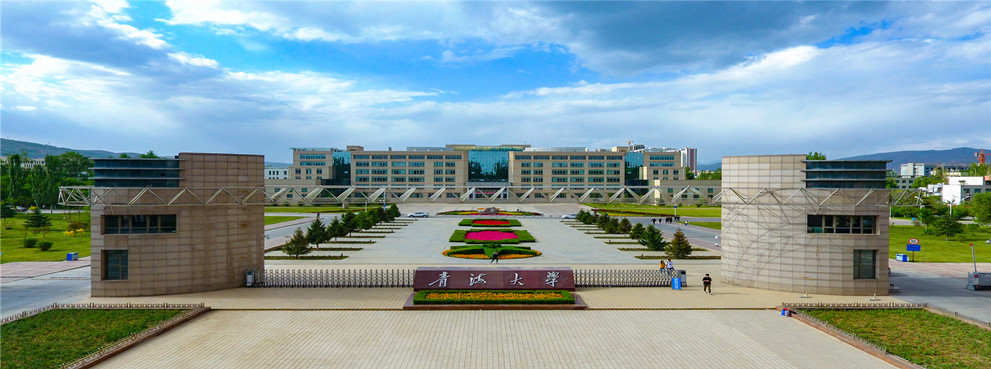
\includegraphics[width=0.618\textwidth]{figure.jpg}%图片名称,放在/figures目录下
	\caption{图片插入\label{fig:fig}}
\end{figure}